\subsection{The Dependency rule} \label{subsec_dependency_rule}

An essential aspect is described as the dependency rule. The rule states that
\textit{source code dependencies must point only inward toward higher-level policies}
(Robert C. Martin, 2018, p. 206). This ’flow of control’ is designed following the
\gls{dip} and can be represented schematically as concentric circles containing all the
components described in section \fullref{subsec_layers} The arrows in Figure
\ref{fig_modulair_components} clearly show that the dependencies flow from the outer
layers to the inner layers. Most outer layers are historically subjected to large-scale
refactorings due to technology changes and innovation. Separating the layers and adhering
to the dependency rule ensures that the domain logic can evolve independently from
external dependencies or certain specific technologies.

\begin{figure}[H]
    \centering
    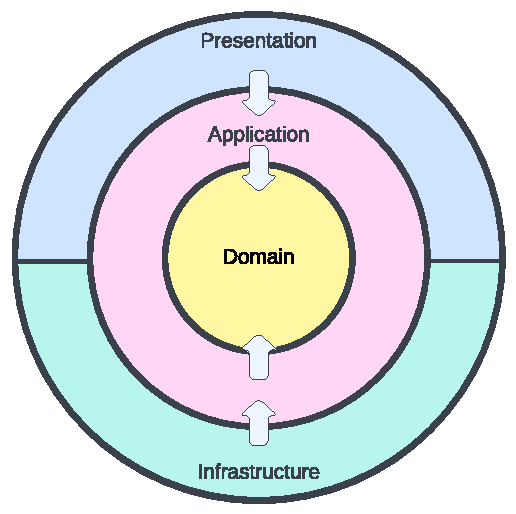
\includegraphics[width=0.4\textwidth]{figures/ca_diagram.pdf}
    \caption[Flow of control]{Flow of control}
    \label{fig_modulair_components}
\end{figure}